\chapter{Evaluation von Werkzeugen zur Softwareverteilung}
\label{cha:evaluation}
Bei der Recherche in Bezug auf mögliche Werkzeuge zur Softwareverteilung im Umfeld von OSGi finden sich mehrere Projekte,
die zum Teil sehr unterschiedliche Zielsetzungen verfolgen.
OpenMUC wird derzeit unter der \ac{GPL} veröffentlicht. Um das Projekt auch weiterhin vollständig frei
nutzen zu können, muss die Komponente zur Softwareverteilung ebenfalls unter einer freien Lizenz stehen.
Aus diesem Grund werden im Weiteren lediglich frei verfügbare Werkzeuge eingehender betrachtet. 

\section{Zu betrachtende Werkzeuge}
\label{werkzeuge}
In einem ersten Schritt werden die recherchierten Werkzeuge vorgestellt und ihre Stärken, Schwächen und Zielsetzungen untersucht.
Den Anfang macht die \acf{OBR}-Implementierung von Apache Felix. Sie bildet die Grundlage für die meisten komplexeren Werkzeuge. 

\subsection{Apache Felix \acs{OBR}}

Eines der grundlegendsten Werkzeuge zur Verteilung von Bundles ist das \ac{OBR}. Spezifiziert wurde es
mit dem \ac{OSGi}-Release 5 im März 2012 \cite[S.529-542]{osgi_r5}. Als Grundlage für die Spezifikation und als Referenzimplementierung 
dient das Apache Felix \ac{OBR}\footnote{\url{http://felix.apache.org/documentation/subprojects/apache-felix-osgi-bundle-repository.html}}.\\

Gédéon \cite{osgi_felix3} beschreibt ein \ac{OBR} als Dienst, der es ermöglicht auf entfernte Archive für Bundles zuzugreifen.
Jedes Archiv (Repository) bietet eine Liste vorhandener Bundles zusammen mit dessen Metadaten an.
Die Metadaten eines Bundles beinhalten zum Beispiel Abhängigkeiten zu anderen Bundles und die im Archiv verfügbaren Versionen eines Bundles.
Der Zugriff erfolgt entweder über eine \ac{API}, oder direkt über eine \ac{XML}-Datei (Repository \ac{XML}), die das Archiv beschreibt.
Die über das Archiv zur Verfügung gestellten Bundles können heruntergeladen und in ein \ac{OSGi}-Framework installiert werden.\\

Die Arbeitsweise mit einem \ac{OBR} ist dabei vergleichbar mit den Installations- und Aktualisierungsvorgängen eines,
auf vorkompilierten Pakten basierenden, Linux Systems.
Es existieren mehrere Quellen für Pakete und für jedes Paket sind seine Abhängigkeiten definiert.
Die Installation und die Aktualisierung von Paketen geht dabei immer vom System selbst aus. 
Damit liegt die Hoheit der Softwareverwaltung beim lokalen System selbst. Das bedeutet für den Einsatz von \ac{OBR}, dass eine Installation oder ein Update für ein Bundle 
lokal angestoßen werden muss. Dies kann interaktiv über eine Shell, wie zum Beispiel über die Felix Gogo-Shell, oder zeitgesteuert über ein Bundle passieren.
In jedem Fall muss der Prozess der Softwareverteilung durch manuelle Schritte, oder über weitere Software in Form eines Bundles ergänzt werden.\\

Seit 2009 existiert mit Apache ACE\footnote{Projektwebseite Apache ACE: \url{https://ace.apache.org}} ein weiteres Werkzeug zur Verteilung von Software für \ac{OSGi}-basierte Anwendungen.

\subsection{Apache ACE}
\glqq The typical use case for using ACE is where you want to control and manage which software runs on what target. \grqq\ \cite{ace}\\

Nach drei Jahren im Incubator\footnote{Den Apache Incubator müssen alle Projekte durchlaufen, die Teil der Apache Software Foundation werden wollen. \url{https://incubator.apache.org/}}
wurde Apache ACE im Jahre 2012 zu einem Top-Level-Projekt der Apache Software Foundation\footnote{Nachricht auf Heise zu Apache ACE: \url{https://heise.de/-1443698}}.
Eines der Hauptprobleme bei modularen Anwendungen wie OpenMUC ist es, bei einer hohen Anzahl an Softwarekomponenten und Installationen den Überblick zu wahren.
Dieses Problem lässt sich mit Hilfe von Apache ACE lösen. Über einen zentralen Apache ACE-Server kann eine große Anzahl an Targets gesteuert und gewartet werden.
Ermöglicht wird dies über drei Teilsysteme, die in Apache ACE integriert sind \cite{ace}:
\begin{enumerate}
 \item \textit{Dependency-management:} Dieses Subsystem dient der Verwaltung von Abhängigkeiten zwischen Artefakten.
 Bei einem Artefakt handelt es sich um eine Komponente, die zum Betrieb des Software-Systems benötigt wird.
 Dabei kann es sich zum Beispiel um ein OSGi-Bundle, oder eine Konfigurationsdatei handeln.
 Zur Verwaltung der Abhängigkeiten werden dien verfügbaren Artefakte zu Features und Features wiederum zu Distributionen zusammengefasst.
 Die Distributionen können auf einem Target installiert werden. Damit lassen sich komplexe Konstellationen von Artefakten abbilden und diese auf eine Vielzahl von Targets installieren.
 \item \textit{Deployment-management:} Dieses Subsystem zur Verteilung der Komponenten sorgt dafür, dass die richtigen Artefakte auf den richtigen Targets installiert werden. 
 Das Subsystem verfügt über Strategien zur Fehlerbehebung, wie der Durchführung von atomaren Updates. %. Eine Strategie stellen zum Beispiel atomare Updates dar.
 Das bedeutet, in einem Fehlerfall wird automatisch der letzte fehlerfreie Zustand wiederhergestellt.
 Außerdem lässt sich die Last beim Deployment auf viele Targets durch den Einsatz von Relay-Server auf einfachem Wege skalieren.
 \item \textit{Feedback-management:} Das Feedback-Subsystem sammelt Informationen, die im Rahmen des Target-Life-Cycle anfallen. Diese werden auf dem zentralen ACE Server aggregiert 
 und können zur Überwachung und weiteren Steuerung der Targets eingesetzt werden.
\end{enumerate}

Eine Apache ACE-Installation ist der klassischen Client-Server-Architektur zuzuordnen. 
Die Installation besteht, wie in \autoref{fig:ace_architecture} zu sehen, aus mindestens einem ACE-Server und einem \ac{OBR}.
Apache ACE verfügt über ein integriertes \ac{OBR} und bietet darüber hinaus die Möglichkeit, externe Archive einzubinden.

\begin{figure}[h]
 \centering
 \includegraphics[width=\textwidth]{../02.Diagramme/tools/ACE_architekture.png}
 \caption{UML-Verteilungsdiagramm der ACE-Architektur}
 \label{fig:ace_architecture}
\end{figure}

Bei einem ACE-Target handelt es sich um ein \ac{OSGi}-Bundle, das entweder in eine bestehende \ac{OSGi}-Anwendung integriert
oder als Stand-Alone-Anwendung betrieben wird. Für jedes ACE-Target existiert eine Konfigurationsdatei, in der mindestens
der Name des Targets und sein Management-Server definiert werden muss.
Sobald das Bundle aktiviert wird, meldet sich das Target bei seinem Management-Server.
Nun können Bundles installiert, aktualisiert und entfernt werden.\\

Mit Karaf\footnote{Projektwebseite Apache Karaf: \url{http://karaf.apache.org}} verfügt die Apache Software Foundation über ein weiteres Werkzeug für das Software-Deployment im Umfeld von \ac{OSGi}.

\subsection{Apache Karaf}
\label{Karaf_1}
Hervorgegangen aus dem Apache ServiceMix Kernel wurde das Projekt im Jahre 2010 zu einem Top-Level-Projekt der
Apache Software Foundation\footnote{Historie des Apache Karaf Projektes: \url{http://icodebythesea.blogspot.de/2011/01/brief-history-of-apache-karaf.html}}.
Der Name orientiert sich an dem Begriff Karaffe, im Englischen carafe, der die Eigenschaften von Apache Karaf treffend beschreibt.
Während eine Karaffe als Behältnis für Wein und andere Getränke genutzt wird, kann Apache Karaf als polymorpher Container für eine 
Vielzahl von Anwendungen genutzt werden.\\

\glqq With this flexibility, Karaf is the perfect solution for microservices, systems integration, big data, and much more. \grqq \cite{karaf}\\

Apache Karaf setzt auf die \ac{OSGi}-Plattform auf und erweitert diese um verschiedene Eigenschaften.
Die folgenden drei Eigenschaften der Karaf-Plattform könnten dabei zur Lösung der Problemstellung dieser Arbeit beitragen \cite{karaf}:

\begin{enumerate}
 \item \textit{Hot-deployment:} Jede Apache Karaf Installation verfügt über einen Hot-deploy\-ment-Ordner. 
 Werden dort Dateien eines unterstützten Formates abgelegt, werden diese automatisch in den Container installiert.
 Dabei unterstützt Karaf neben \ac{OSGi}-Bundles auch Aries\footnote{Projektwebseite Aries: \url{http://aries.apache.org}}-Blueprint-Bundles, 
 Spring\footnote{Projektwebseite Spring: \url{http://spring.io/}}-\ac{XML}-, \ac{KAR}-, sowie \ac{WAR}- und \ac{WAB}-Dateien.
 
 \item \textit{Provisioning:} Artefakte können der Karaf-Plattform auf viele Arten zur Verfügung gestellt werden. Neben dem Einsatz eines \ac{OBR} können
 die Artefakte z.B. über ein maven-Repository, als lokale Datei oder über das \ac{HTTP}, bzw. über das \ac{HTTPS} in die Plattform eingebunden werden. 
 Des Weiteren verfügt Karaf über das Konzept der Karaf Features, auf die im Anschluss detaillierter eingegangen wird.
 
 \item \textit{Management:} Der Karaf-Container bietet eine Vielzahl von Informationen, die für die Überwachung und die Steuerung des Containers eingesetzt
 werden können. Die Überwachung und Steuerung des Containers erfolgt mit Hilfe von \ac{JMX}. Mit dem Karaf Decanter existiert bereits eine 
 Anwendung zur Überwachung und Steuerung eines Karaf-Containers. Über \ac{JMX} ist es jedoch unkompliziert möglich, eigene Management-Anwendungen zu entwickeln.
\end{enumerate}

\textit{Karaf Feature:}\\
\glqq As a lightweight and standalone \ac{OSGi} container, Apache Karaf proposes another way to provision applications.
Apache Karaf Features is the default provisioning solution in Apache Karaf. \grqq\ \cite{learning_karaf_cellar}\\

Bei einem Karaf Feature handelt es sich also um eine Zusammenstellung von Softwarekomponenten für die Karaf-Plattform.
Onofré beschreibt ein Karaf Feature als Anwendung, bestehend aus Bundles, anderen Karaf Features und der Konfiguration, 
die für die Anwendung notwendig ist \cite{learning_karaf_cellar}.
Ein verfügbares Feature wird in einem vorgegebenen \ac{XML}-Format beschrieben. Es ist möglich, mehrere Features in derselben Datei zu
definieren. Man spricht dann von einem Feature Repository. Ein Beispiel für eine OpenMUC Karaf-Anwendung ist in 
\autoref{fig:karaf_feature} zu sehen. Das Feature-Repository beschreibt zwei Features.
Zum einen das openmuc-external-Feature, das in Zeile 2 der Abbildung beschrieben wird und aus zwei Bundles besteht.
Zum anderen wird in Zeile 7 das openmuc-core-Feature spezifiziert.
Bei Verweisen auf die Bundles ist Karaf nicht auf das lokale Dateisystem beschränkt.

\begin{figure}[h]
 \centering

 \lstinputlisting[language=XML]{content/sourcecode/karaf.xml}
 \caption{Minimale XML-Datei für ein OpenMUC Feature-Repository}
 \label{fig:karaf_feature}
\end{figure}

Wie in Zeile 3 und 4 der \autoref{fig:karaf_feature} zu sehen, ist es ohne Weiteres möglich, entfernte Bundles einzubinden.
Das erste Bundle des openmuc-external-Feature wird über \ac{HTTP}, das zweite wird über das MVNRepository eingebunden.
Das openmuc-core-Feature besteht aus dem openmuc-external-Feature und zwei lokal verfügbaren Bundles, welche in Zeile 9 und 10 beschrieben werden.
Des Weiteren können Konfigurationsdateien (Zeile 11) angeben werden, die innerhalb der Anwendung benötigt werden.\\

Über das Konzept der Karaf Features lassen sich beliebig komplexe und modulare Anwendungen für Karaf beschreiben.
Dadurch können verschiedene Kompositionen des OpenMUC-Frameworks, je nach Anwendungsfall und Anforderung, zusammengestellt werden.
Als letztes Werkzeug wird im Folgenden Eclipse hawkBit\footnote{Projektwebseite Eclipse hawkbit: \url{https://eclipse.org/hawkbit/}} vorgestellt.

\subsection{Eclipse hawkBit}

\glqq Das von Bosch Software Innovations initiierte Eclipse hawkBit-Projekt hat sich zum Ziel gesetzt,
eine domänenunabhängige und offene Plattform für Software-Updates im IoT-Kontext bereitzustellen. \grqq \cite{heise_hawkbit}\\

Bei hawkBit liegt der Fokus auf der Verteilung von Software und Updates. Über die Beschaffenheit der verschiedenen Artefakte 
weiß hawkBit nur das Nötigste. In diesem Punkt unterscheidet sich hawkBit deutlich von Apache ACE. Während ACE die Abhängigkeiten
von Bundles selbständig auflösen kann, ist man beim Einsatz von hawkBit selbst in der Pflicht, die für eine Anwendung benötigten Artefakte zu verteilen.
Ziel von hawkBit ist es, eine generische Lösungen für das Problem der Software- und Update-Verteilung in allen \ac{IoT}-Domänen bereitzustellen.\\

Die Kommunikation mit den Geräten erfolgt entweder direkt oder über eine Device-Mangement-\ac{API}.
Neue Protokolle zur direkten Kommunikation können durch die Implementierung eines entsprechenden Adapters auf einfachem Wege integriert werden.
Des Weiteren ist es möglich, zur Kommunikation mit den Geräten auf einen Device-Management-Dienst aus dem \ac{IoT}-Umfeld zurückzugreifen. 
Derzeit werden die Protokolle \ac{OMA-DM} und \ac{LWM2M} unterstützt. Eclipse hawkBit verfügt über zwei interessante Eigenschaften, welche für die 
Zielsetzung dieser Arbeit von Bedeutung sind und im Folgenden eingehend beschrieben werden \cite{hawkbit}:

\begin{enumerate}
 \item \textit{Rollout-Management:} Das Rollout-Management ist für eine große Anzahl von Targets konzipiert und lässt sich durch 
 den Einsatz weiterer Rollout-Server horizontal skalieren. Der Rollout-Prozess wird fortlaufend überwacht. Dies ermöglicht es, den genauen Zustand des Prozesses zu
 jedem Zeitpunkt zu ermitteln. Des Weiteren ist es möglich, die Targets in verschiedene Gruppen aufzuteilen und den Rollout-Prozess kaskadierend zu gestalten. 
 Dabei wird die Installation von Software auf eine nachfolgende Gruppe von Targets erst dann gestartet, wenn in der vorangegangenen Gruppe ein definierter Schwellenwert erreicht wird.
 Als Schwellenwert kann eine Erfolgsbedingung oder eine Fehlerbedingung zum Einsatz kommen.
 Die Erfolgsbedingung wird anhand eines festgelegten prozentualen Anteils erfolgreicher Installationen definiert.
 Die Fehlerbedingung wird über den prozentualen Anteil fehlerhafter Installationen ausgedrückt. 
 Erreicht eine Gruppe von Targets eine definierte Fehlerrate, wird der Prozess abgebrochen und eine Notfallabschaltung eingeleitet. 
 
 \item \textit{Package-Model: } Ein Software-Update besteht meistens aus mehreren Teilen, wie Laufzeitkomponenten, Anwendungskomponenten und Konfigurationsdateien \cite{jaxenter_hawkbit}. 
 Eclipse hawkBit verfügt mit dem Package-Model über ein ähnliches Konzept wie das, in \autoref{Karaf_1} beschriebene, Karaf Feature.
 Das Datenmodell besteht, wie in \autoref{fig:hawkbit_packagemodel} zu sehen, aus mehreren Bausteinen. Zunächst werden mehrere Artefakte, 
 wie z.B. \ac{OSGi}-Bundles oder Konfigurationsdateien, zu einem Software-Modul vereint. Dieses Software-Modul kann mit zusätzlichen Metadaten, wie einer Versionsnummer und verschiedenen 
 Schlüsselworten, versehen werden. In einem nächsten Schritt werden die einzelnen Software-Module zu einem Distribution-Set zusammengesetzt.
 Für das Distribution-Set können ebenfalls verschiedene Metadaten hinterlegt werden.
 So können auf einem Target mehrere Software-Module in Form eines Distribution-Set in einem atomaren Update-Prozess eingespielt werden \cite{jaxenter_hawkbit}.
\end{enumerate}

\begin{figure}[h]
 \centering
 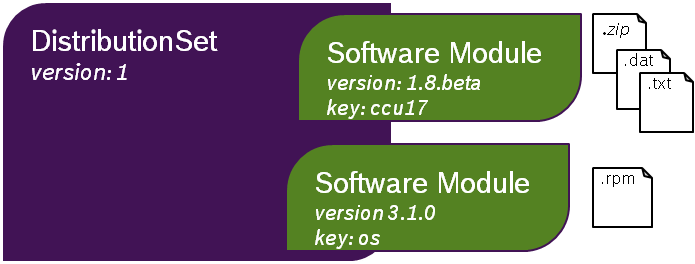
\includegraphics[scale=0.55]{content/pictures/hawkbit_packagemodel.png}
 \caption{HawkBit Package Model \cite{jaxenter_hawkbit}}
 \label{fig:hawkbit_packagemodel}
\end{figure}

Momentan steht das hawkBit-Projekt noch am Anfang seiner Entwicklung, was auch an der jungen Versionsnummer 0.2.0 abzulesen ist.
Dies bedeutet aber nicht, dass die Software nicht produktiv eingesetzt werden kann.
Durch den starken Fokus auf die Basisfunktionalität, der Definition klarer Schnittstellen und nicht zuletzt durch die starke Unterstützung der Firma Bosch,
ist in sehr kurzer Zeit ein mächtiges Werkzeug zur Softwareverteilung und Softwareaktualisierung entstanden.\\

Bevor die in diesem Kapitel vorgestellten Werkzeuge bewertet werden, müssen entsprechende Kriterien zur Bewertung ermittelt werden.
Dafür werden im nächsten Abschnitt Einsatzszenarien vorgestellt und diese auf verschiedene Anforderungen für die Softwareverteilung hin untersucht.

\section{Einsatzszenarien des OpenMUC-Frameworks}
\label{sec:openmuc_scenarios}

Dieses Kapitel dient der Ermittlung von Anforderungen, die an ein Werkzeug zur Softwareverteilung für OpenMUC gestellt werden.
Dazu werden im Folgenden verschiedene Einsatzszenarien des OpenMUC-Frameworks in aktuellen Forschungsprojekten beschrieben.
Diese Szenarien werden um eine Komponente zur Verwaltung der OpenMUC-Installationen erweitert,
um mögliche Anforderungen an ein Werkzeug zur Softwareverteilung zu identifizieren.\\

Zu den Hauptaufgaben des OpenMUC-Frameworks zählt zum einen die Überwachung von Anlagen und Geräten und zum anderen das Aufzeichnen von dort anfallenden Messwerten.
So auch im Projekt Basel Monitoring. Bei diesem Projekt ging es um die Überwachung verschiedener Sensoren einer komplexen Heizanlage und der Protokollierung der Sensorwerte.
Bei der geforderten Funktionalität handelt es sich um die Kernkompetenzen des OpenMUC-Frameworks.
In der Regel müssen dafür keine zusätzlichen Softwarekomponenten entwickelt und verteilt werden.
Voraussetzung dafür ist, dass die benötigten Protokolle und Treiber für OpenMUC existieren.
Wie in \autoref{fig:openmuc_basel} zu sehen, ist die Topologie dieses Szenarios einfach gehalten. Eine OpenMUC-Installation 
ist direkt mit den verschiedenen Sensoren des Heizsystems verbunden.

\begin{figure}[h]
 \centering
 \includegraphics[scale=0.23]{../02.Diagramme/scenarios/basel_v2.png}
 \caption{OpenMUC Projekt Basel Monitoring}
 \label{fig:openmuc_basel}
\end{figure}

Hierbei handelt es sich um eine passive Installation, die nicht steuernd in den Betrieb der Heizanlage eingreift. 
Wichtig an dieser Stelle ist die möglichst lückenlose Aufzeichnung der Messdaten.
Aus diesem Grund muss der fehlerfreie Betrieb der OpenMUC-Installation von zentraler Stelle überwacht werden.\\

Deutlich komplexer gestaltetet sich das Projekt Fellbach ZEROplus\footnote{\url{https://www.ise.fraunhofer.de/de/forschungsprojekte/fellbach-zeroplus.html}}.
Hierbei handelt es sich um eine, durch das \ac{BMVI} geförderte Feldstudie zur Erprobung eines Heimenergie-Managementsystems.
Hierfür wurde auf Basis von OpenMUC eine smarte Energiesteuerung umgesetzt.
Diese ermittelt auf Basis von aktuellen Messwerten und Prognosen, basierend auf historischen Daten, zum einen den zu erwartenden Ertrag der PV-Anlage und zum 
anderen den Verbrauch des Haushaltes innerhalb der nächsten Stunden \cite{fellbach}.
Auf Grundlage dieser Daten werden verschiedene Verbraucher und Speicher gesteuert, mit dem Ziel den Verbrauch des selbst produzierten Stroms zu erhöhen und bei Überschüssen 
zu speichern. Wie in \autoref{fig:openmuc_fellbach} dargestellt, ist dafür eine komplexere Topologie notwendig.
OpenMUC bildet an dieser Stelle eine Brücke zwischen den beiden \ac{IoT}-Domänen Smart-Energy und Smart-Grid.

\begin{figure}[h]
 \centering
 \includegraphics[scale=0.23]{../02.Diagramme/scenarios/fellbach_v2.png}
 \caption{OpenMUC Projekt Fellbach ZEROplus}
 \label{fig:openmuc_fellbach}
\end{figure}

Neben der Auswertung verschiedenster Sensordaten und der Steuerung von Anlagen und Geräten des Smart-Home, muss die OpenMUC-Plattform 
aufwendige algorithmische Aufgaben bewältigen. Im Rahmen des Projektes wurden mehrere Energieplushäuser mit einem Heimenergie-Managementsystem ausgestattet.
Die dabei zum Einsatz kommenden Verbraucher und Speicher können von Haus zu Haus variieren. Das bedeutet, dass die eingesetzten Softwarekomponenten 
zwischen den OpenMUC-Installationen variieren. Das wiederum hat Konsequenzen für den Einsatz eines Werkzeuges zur Softwareverteilung. 
Neben einer Basis-Distribution für das gesamte Projekt, müssen verschiedene Konstellationen von Komponenten für jedes Haus definiert werden können.
OpenMUC übernimmt in diesem Projekt eine aktive Steueraufgabe. Aus diesem Grund gewinnt an dieser Stelle das Thema Sicherheit an Bedeutung. 
Durch die Etablierung einer Softwareverteilung ist mit Angriffen, wie sie in \autoref{sicherheit} beschrieben werden, zu rechnen.\\

Das Projekt CheapFlex\footnote{\url{http://forschung-stromnetze.info/projekte/guenstige-smart-grids-mit-rundsteuertechnologie/}} ist ein Forschungsvorhaben aus dem Bereich der Smart-Grids.
Ziel des Projektes ist es, ganze Netzstränge zu dynamisieren, um so auf Engpässe oder Überangebote im Stromnetz reagieren zu können. 
Die momentan festgelegten Hoch- und Niedertarife entsprechen nicht mehr den Anforderungen des, durch die regenerativen Energien, veränderten Stromnetzes.
Zur Dynamisierung wird über ein Tonfrequenz-Rundsteuersignal der aktuelle Stromtarif über die Stromleitung übertragen.
Auf Grundlage dieses Signals werden durch OpenMUC verschiedene Erzeuger, Verbraucher und Speicher geregelt.
Die \autoref{fig:openmuc_cheapflex} skizziert den Aufbau eines einzelnen Netzstranges.
Das Tarifsignal wird von einer Leitwarte aus in den Netzstrang eingespeist. Des Weiteren überwacht die Leitwarte Angebot und Nachfrage innerhalb des Netzstranges
und kann in Ausnahmesituationen die verschiedenen Erzeuger, Verbraucher und Speicher direkt steuern.

\begin{figure}[h]
 \centering
 \includegraphics[scale=0.23]{../02.Diagramme/scenarios/cheapflex_v2.png}
 \caption{OpenMUC Projekt CheapFlex}
 \label{fig:openmuc_cheapflex}
\end{figure}

Auch in diesem Projekt ist die Sicherheit eine der zentralen Anforderungen und das nicht nur in Bezug auf die Einführung eines Werkzeuges zur Softwareverteilung.
Sicherheitsupdates müssen zeitnah und ohne weiteres Gefährdungspotential verteilt werden können.
Zusätzlich ist eine zentrale Überwachung der Softwarestände und der Betriebsfähigkeit bei der Vielzahl der OpenMUC-Installationen unabdingbar.\\

Das letzte Szenario beschreibt den Einsatz von OpenMUC im Smart-Home-Labor der Hochschule Furtwangen.
\autoref{fig:sh_lab} zeigt eine mögliche Topologie des Smart-Home-Labors nach der Integration von OpenMUC und einem Server für die Softwareverteilung.

\begin{figure}[h]
 \centering
 \includegraphics[scale=0.23]{../02.Diagramme/scenarios/sh_lab.png}
 \caption{Smart-Home-Labor der Hochschule Furtwangen}
 \label{fig:sh_lab}
\end{figure}

Im Gegensatz zum Bereich Smart-Energy herrscht im Smart-Home eine deutlich höhere Diversität und Fluktuation bei den verfügbaren Sensoren und Aktoren. In den bereits dargestellten Szenarien 
sind die zum Einsatz kommenden Aktoren, wie \acp{BHKW}, Ladesäulen für Elektroautos und Wärmepumpe meist zu Beginn bekannt und werden selten verändert.
Im Bereich des Smart-Home liegt der Fokus auf einer einfachen und schnellen Integration von Things in die Gesamtinfrastruktur. Hinzu kommen mobile Geräte, die nur 
bei physikalischer Nähe in das Smart-Home integriert werden, zum Beispiel durch das Einbuchen in ein \ac{WLAN}.
Ein weiterer Fokus liegt im Zusammenspiel verschiedener Gateways und der Anbindung an proprietäre Protokolle.
Ziel des Labors ist es, verschiedene Anwendungsfällen im Smart-Home-Umfeld zu erproben. 
Dadurch ergibt sich zum einen die Anforderung, möglichst einfach neue Things in OpenMUC zu integrieren und zum anderen mit wenig Aufwand
die Anwendungsfälle und Routinen der OpenMUC-Installation auszutauschen. \\

Anhand dieser Einsatzszenarien lassen sich bereits einige Anforderungen an ein Werkzeug zur Verwaltung der Softwarestände der OpenMUC-Installationen ableiten.
Trotz der Unterschiede innerhalb der Szenarien ergeben sich einige Überschneidungen innerhalb der Anforderungen.
Neben der Sicherheit ist die zentrale Verwaltung der Installationen eine primäre Anforderung an ein Werkzeug zur Softwareverteilung. 
Im Projekt CheapFlex besteht die Anforderung, dass Systeme von Dritten mit dem Werkzeug interagieren müssen. 
Aus diesem Grund sollte das Werkzeug zur Softwareverteilung über Schnittstellen zur Überwachung und Steuerung der angebundenen OpenMUC-Installationen verfügen.
In den oben genannten Feldstudien werden die OpenMUC-Gateways häufig über das Handynetz oder über \ac{WLAN} mit dem Internet verbunden.
Vor allem dann, wenn ein Gateway über das Handynetz mit neuer Software versorgt wird, ist eine Unterbrechung der Verbindung nicht unwahrscheinlich.
In diesem Fall müssen die zu untersuchenden Werkzeuge über geeignete Strategien verfügen, um mit dieser Unterbrechung umzugehen.
Im Folgenden wird die in diesem Abschnitt ermittelte Sammlung von Anforderungen erweitert und näher erläutert.

\section{Kriterien zur Bewertung der Werkzeuge}

Für die Bewertung der zu untersuchenden Werkzeuge aus \autoref{werkzeuge} wird in diesem Abschnitt ein Katalog von Kriterien definiert.
Dazu wurden aus den im vorherigen Abschnitt gewonnenen Anforderungen die Kriterien Nr. 1 bis einschließlich Nr. 6 abgeleitet.
Ergänzt wurde der Katalog um weitere Kriterien (Nr. 7 -11) zur Auswahl von Open-Source-Software, aus der Arbeit von Cruz et al. \cite{evaluation_criteria}. 


\begin{enumerate}[label={Nr. \arabic*}, leftmargin=*, labelindent=1em]
 \item Sicherheit: Die Software ist in Bezug auf die drei Sicherheitsaspekte aus \autoref{sicherheit} zu bewerten.
 
 \item Zentrales Management: Das Werkzeug verfügt über Fähigkeiten zur zentralen Verwaltung mehrerer Targets. Darunter fällt die Überwachung der Betriebsbereitschaft
 des Targets und die Überwachung seiner Softwarekomponenten.
 
 \item Distributionen: Es ist möglich, verschiedene Konstellationen von Softwarekomponenten zu definieren und im Ganzen auf ein Target aufzuspielen. 

 \item Ausfallsicherheit: Die Software verfügt über Strategien zur Fehlerbehebung. Die Targets befinden sich nach Fehlern bei der Installation
 oder nach einem Verbindungsabbruch in einem vorhersagbaren Zustand.
 
 \item Schnittstellen (\ac{API}): Das Werkzeug verfügt über Schnittstellen, die es Software Dritter ermöglicht, Daten auszulesen und 
 Befehle zur Steuerung abzusetzen.
 
 \item Zielplattform \ac{OSGi}: Das Werkzeug ist auf die Verteilung von Softwarekomponenten für Anwendungen, basierend auf der \ac{OSGi}-Plattform, spezialisiert.

 \item Existierende Community \cite{evaluation_criteria}: Es existieren Personen, in Form von Nutzern 
  und Entwicklern, die kontaktiert werden können.
  Das Projekt verfügt über Kommunikationskanäle und Plattformen, um mit diesen Personen Kontakt aufnehmen zu können.
 
 \item Erkennbare Weiterentwicklung \cite{evaluation_criteria}: Die Software wird kontinuierlich gepflegt. 
  Bekanntgewordene Fehler werden behoben und es existiert ein Plan, zum Beispiel eine Roadmap, für die zukünftige Weiterentwicklung der Software.
 
 \item Langlebiges Projekt \cite{evaluation_criteria}: Das Projekt und seine Community existieren bereits über einen längeren Zeitraum.
 
 \item Flexible Wartbarkeit \cite{evaluation_criteria}: Die Software kann an eigene Anforderungen angepasst werden.
 
 \item Anzahl Entwickler \cite{evaluation_criteria}: Die Anzahl an Entwicklern, die in das Projekt involviert sind. Für diese Arbeit werden nur Entwickler 
 gezählt, die in den Jahren 2016 und 2017 mehr als fünf Code-Einreichungen aufweisen können.
\end{enumerate}

Im nächsten Schritt ist für jedes Kriterium ein möglicher Wertebereich für die Bewertung festzulegen.
Dabei wird bei der Bewertung zwischen zwei Arten von Kriterien unterschieden.
Zum einen Kriterien, die auf einer relativen Skala von einem Punkt bis zu vier Punkte bewertet werden und
zum anderen Kriterien, bei denen die Verfügbarkeit (ja), bzw. Nichtverfügbarkeit (nein) bewertet wird. 
Die vollständige Katalog der Kriterien mit den entsprechenden Wertebereichen ist in \autoref{tab:anforderungsliste} zu sehen.\\

\begin{table}[H]
 \centering
 \caption{Kriterienkatalog und Wertebereich der einzelnen Kriterien}
 \begin{tabular}{c|l|l}
 \multicolumn{3}{l}{}\\
  \multicolumn{3}{l}{\textbf{Kriterien}}\\
  \multicolumn{3}{l}{}\\
  \toprule
  Nr. &  Kriterium & Wertebereich \\
  \midrule
  1 & Sicherheit 
  & 1 - 4 \\
  
  2 & Zentrales Management 
  & ja, nein \\
  
  3 & Distributionen
  & ja, nein \\
  
  4 & Ausfallsicherheit
  & ja, nein\\
  
  5 & Schnittstellen (\ac{API})
  & ja, nein\\
  
  6 & Zielplattform OSGi
  & ja, nein\\
  
  7 & Existierende Community
  & ja, nein \\
  
  8 & Erkennbare Weiterentwicklung 
  & 1 - 4\\
  
  9 & Langlebiges Projekt 
  & 1 - 4\\
  
  10 & Flexible Wartbarkeit 
  & 1 - 4\\
  
  11 & Anzahl Entwickler 
  & 1 - 4\\
  \bottomrule
 \end{tabular}
 \label{tab:anforderungsliste}
\end{table}

Im Anschluss erfolgt die Bewertung der einzelnen Werkzeuge bezogen auf die in diesem Abschnitt definierten Kriterien.

\section{Evaluation der einzelnen Werkzeuge}
\label{sec:rating}

Dieses Kapitel schafft die Grundlage für die spätere Auswahl eines geeigneten Werkzeuges. Jedes Werkzeug wird 
auf die definierten Kriterien hin untersucht und bewertet. Bei dem Kriterium Nr. 1 Sicherheit wird 
unter anderem die Anzahl an Einträgen, in der \ac{CVE}\footnote{\url{https://cve.mitre.org/}}-Datenbank einbezogen.
Zusätzlich wird für jedes Werkzeug ein einheitlicher Steckbrief in tabellarischer Form erstellt. Diese tragen 
zu einer besseren Übersicht und leichteren Vergleichbarkeit der Werkzeuge bei. 
Als erstes erfolgt die Bewertung der Apache Felix Implementierung der \ac{OBR}-Spezifikation.

\subsection{Apache Felix OBR}

Im folgenden wird das Apache Felix OBR, hinsichtlich der elf definierten Kriterien bewertet.

\begin{enumerate}[label={Nr. \arabic*}, leftmargin=*, labelindent=1em]
 \item Sicherheit:
 Zum jetzigen Zeitpunkt sind keine Sicherheitslücken oder anderweitige Schwachstellen für die Apache Felix OBR Implementierung bekannt.
 Der Zugriff auf ein Repository kann über \ac{HTTP}, \ac{HTTPS} und das lokale Dateisystem erfolgen.
 Werden nur lokale Repositories oder solche die \ac{HTTPS} anbieten genutzt, kann die Gefahr durch \ac{MITM}-Angriffe reduziert werden.
 Zur Signierung der Bundles kann nur die in der \ac{OSGi}-Spezifikation definierte Methode eingesetzt werden. 
 Die Client-Implementierung von \ac{OBR} beschränkt sich auf ein Minimum an Funktionalität und bietet deshalb nur wenig Fläche für Angriffe.
 Das Einbinden von unbekannten Fremdquellen birgt natürlich ein Risiko, da sowohl die Informationen des Repositories, als auch die Bundles auf Seite des 
 Clients verarbeitet werden müssen.
 Dieses Risiko besteht aber bei allen zu betrachtenden Werkzeugen.
 Aus diesen Gründen werden für das Kriterium Sicherheit vier Punkte vergeben.
 
 \item Zentrales Management: 
 Ein \ac{OBR} entspricht der Client-Server-Architektur, wobei alle Aktionen ihren Ursprung im Client haben.
 Es bietet keine Möglichkeiten zur zentralen Verwaltung mehrerer Targets.
 
 \item Distributionen:
 Das \ac{OBR} arbeitet mit Bundles. Die Komposition mehrerer Bundles ist nicht vorgesehen und wird nicht unterstützt.
 
 \item Ausfallsicherheit:
 Die Client-Implementierung sieht keine Strategien zur Fehlerbehandlung vor. Dies obliegt dem Prozess, der die Installation eines Bundles per 
 \ac{OBR} initiiert und überwacht. Auch die Auflösung von Abhängigkeiten und die Installation selbiger fällt nicht in den Aufgabenbereich des \ac{OBR}.
 
 \item Schnittstellen (\ac{API}):
 Es existieren Schnittstellen auf der Ebene von \ac{OSGi}. Dadurch ist es möglich, in anderen Bundles die Funktionalität der \ac{OBR}-Implementierung zu nutzen.
 Anhand dieser Schnittstellen wäre es zum Beispiel möglich, einen Management-Agent zu entwickeln, der Strategien zur Fehlerbehandlung und zur Auflösung von Abhängigkeiten
 bereit stellt.
 
 \item Zielplattform \ac{OSGi}: Das Werkzeug wurde zur Verteilung von \ac{OSGi}-Bundles entwickelt.
 
 \item Existierende Community:
 Da es sich um ein Teilprojekt des Apache Felix Projektes handelt, können auch die selben Personen kontaktiert werden.
 Es existieren mehrere Mailinglisten\footnote{Apache Felix Mailinglisten: \url{http://felix.apache.org/mailinglists.html}} um mit den Benutzern und den Entwicklern 
 in Kontakt zu treten. Die Mailinglisten werden regelmäßig frequentiert, was eine aktive Community vermuten lässt.
 
 \item Erkennbare Weiterentwicklung:
 Das Apache Felix \ac{OBR} gilt als Vorlage für die \ac{OSGi}-Spezifikation und als Referenzimplementierung.
 Seit der Aufnahme in das \ac{OSGi}-Release 5 wurde an der Spezifikation nichts mehr geändert. Es existieren auch keine Pläne, 
 die Funktionalität des \ac{OBR} zu erweitern.
 Aus diesem Grund wird für dieses Werkzeug ein Punkt vergeben.
 
 \item Langlebiges Projekt:
 An dieser Stelle wird die Langlebigkeit des Hauptprojektes bewertet.
 Seit Juli 2006\footnote{Nachrichten des Apache Felix-Projektes: \url{http://felix.apache.org/news.html}} ist Apache Felix ein Top-Level-Projekt der Apache Software Foundation. 
 Das Apache Felix-Projekt wird bis zum heutigen Zeitpunk stetig weiterentwickelt und verfügt über eine aktive Community.
 Im Vergleich mit den anderen Werkzeugen handelt es sich um das älteste Projekt und erhält deshalb eine Bewertung von vier Punkten.
 
 \item Flexible Wartbarkeit:
 Das \ac{OBR} ist Teil des \ac{OSGi}-Standards und damit nicht veränderbar. Allerdings ist es über die verfügbaren Schnittstellen möglich, 
 die Funktionalität mit eigenen Bundles zu erweitern.
 Das ermöglicht die höchste Flexibilität unter den zu bewertenden Werkzeugen. Daher werden für dieses Kriterium vier Punkte vergeben.
 
 \item Anzahl Entwickler:
 Die Daten wurden dem Git-Repository\footnote{Apache Felix Sourcecode-Archiv:\url{https://github.com/apache/felix}} des Projektes entnommen.
 Demnach verfügt das Projekt derzeit über acht aktive Entwickler und liegt damit an zweiter Stelle. 
 Das führt im Vergleich mit den anderen Werkzeugen in diesem Kriterium zu zwei Punkten.
 
 
\end{enumerate}

In \autoref{tab:rating_obr} sind die wichtigsten Informationen und die Bewertung nochmals in Form eines Steckbriefes zusammengefasst.

\begin{table}[H]
 \centering
 \caption{Steckbrief: Apache Felix OBR}
 \begin{framed}
 \begin{tabular}{l|l|l|l}
  \multicolumn{4}{l}{}\\
  \multicolumn{4}{l}{\textbf{Apache Felix OBR}}\\
  \multicolumn{4}{l}{}\\
  \toprule
  %Nr. &  Anforderung & Wertebereich \\
  %\midrule
  \multicolumn{2}{l|}{Webseite des Projektes} & \multicolumn{2}{p{8cm}}{\url{https://felix.apache.org}}\\
  
  \multicolumn{2}{l|}{} & \multicolumn{2}{l}{}\\
  
  \multicolumn{2}{l|}{Beginn der Entwicklung} & \multicolumn{2}{p{8cm}}{Januar 2008\footnotemark}\\
  
  \multicolumn{2}{l|}{} & \multicolumn{2}{l}{}\\
  
  \multicolumn{2}{l|}{Stand Entwicklung} & \multicolumn{2}{p{8cm}}{Aktuelle Version: 2.0.2 vom 26.06.2014} \\
  
  \multicolumn{2}{l|}{} & \multicolumn{2}{l}{} \\
  
  \multicolumn{2}{l|}{Beschreibung} &  \multicolumn{2}{p{8cm}}{
  Apache Felix OBR ist die Referenzimplementierung der OSGi-Repository-Service-Specification. Diese ermöglicht die Nutzung von Repositories zur Installation von Bundles.
  } \\
  
  \multicolumn{2}{l|}{} & \multicolumn{2}{l}{} \\
  
  \multicolumn{2}{l|}{Schwerpunkt} &  \multicolumn{2}{p{8cm}}{
  Vereinfacht die Verteilung und Nutzung von Bundles durch zentrale Repositories. 
  Ermöglicht es, Bundles über einen definierten Dienst mit anderen zu teilen und fördert damit die unabhängige Entwicklung von Bundles.
  } \\
  
  \multicolumn{2}{l|}{} & \multicolumn{2}{l}{} \\
  
  \multicolumn{2}{l|}{Besondere Features} & \multicolumn{2}{p{8cm}}{keine} \\
  
  \multicolumn{4}{l}{} \\
  
  Nr. &  \multicolumn{2}{l|}{Kriterium} & Bewertung \\
  \midrule
  1 & \multicolumn{2}{l|}{Sicherheit}
  & 4 \\
  
  2 & \multicolumn{2}{l|}{Zentrales Management}
  & nein \\
  
  3 & \multicolumn{2}{l|}{Distributionen}
  & nein \\
  
  4 & \multicolumn{2}{l|}{Ausfallsicherheit}
  & nein \\
  
  5 & \multicolumn{2}{l|}{Schnittstellen (\ac{API})}
  & ja \\
  
  6 & \multicolumn{2}{l|}{Zielplattform OSGi}
  & ja \\
  
  7 & \multicolumn{2}{l|}{Existierende Community}
  & ja \\
  
  8 & \multicolumn{2}{l|}{Erkennbare Weiterentwicklung}
  & 1 \\
  
  9 & \multicolumn{2}{l|}{Langlebiges Projekt}
  & 4 \\
  
  10 & \multicolumn{2}{l|}{Flexible Wartbarkeit}
  & 4 \\
  
  11 & \multicolumn{2}{l|}{Anzahl Entwickler}
  & 2 \\
  \bottomrule
 \end{tabular}
 \label{tab:rating_obr}
 \end{framed}
\end{table}

\footnotetext{Erstes Felix OBR-Release: \url{https://mvnrepository.com/artifact/org.apache.felix/org.osgi.service.obr/1.0.0}}

Im Folgenden wird das Werkzeug Apache ACE, hinsichtlich der definierten Kriterien bewertet.

\subsection{Apache ACE}

\begin{enumerate}[label={Nr. \arabic*}, leftmargin=*, labelindent=1em]
 \item Sicherheit:
 Zum jetzigen Zeitpunkt sind keine Sicherheitslücken oder anderweitige Schwachstellen für Apache ACE bekannt.
 Zum Schutz der Kommunikation kann \ac{SSL} eingesetzt werden\footnote{Konfiguration der Zwei-Wege-SSL-Authentifizierung \url{https://ace.apache.org/docs/using-client-certificates.html}}.
 Dadurch wird die Kommunikation zwischen Target und ACE-Server über eine Zwei-Wege-\ac{SSL}-Authentifizierung abgesichert.
 Zur Signierung der Bundles kann lediglich die in der \ac{OSGi}-Spezifikation definierte Methode eingesetzt werden. 
 Bundles können nur durch einen Administrator in das interne \ac{OBR} aufgenommen werden. Das erhöht die Sicherheit der Targets in Bezug auf 
 kompromittierte Bundles. Der Apache ACE-Server verfügt über mehrere Schnittstellen, die zur Kommunikation mit seiner Umwelt genutzt werden.
 Diese sind zwar durch ein System zur Authentifizierung und Autorisierung geschützt, bieten aber trotzdem Angriffsmöglichkeiten.
 Die Gefahr vor \ac{MITM}-Angriffen und bösartigen Bundles kann durch die in Apache ACE getroffenen Maßnahmen reduziert werden. Allerdings
 bietet der Server einige Angriffsflächen. Bei Software dieser Komplexität ist davon auszugehen, dass Fehler und Schwachstellen im Code existieren.
 Aus diesen Gründen wird die Sicherheit bei Apache ACE mit drei Punkten bewertet.
 
 \item Zentrales Management: 
 Apache ACE ist für den Zweck der zentralen Verwaltung von Software und deren Verteilung entwickelt worden. 
 
 \item Distributionen:
 Apache ACE ermöglicht es, Artefakte zu komplexen Distribution zusammenzustellen. Dabei bestehen die Distributionen nicht direkt aus Artefakten, sondern aus Features.
 Ein Feature wiederum besteht aus mehreren Artefakten. Dabei gilt, ein Artefakt kann ein Teil mehrerer Features sein, ein Feature kann ein Teil mehrerer Distributionen sein und 
 auf einem Target können mehrere Distribution installiert werden.
 
 \item Ausfallsicherheit:
 Änderungen wie Updates oder die Installation von Bundles werden als atomare Einheit durchgeführt. Tritt bei einer Änderung am Target ein Fehler auf, wird der letzte 
 Zustand wiederhergestellt.
 
 \item Schnittstellen (\ac{API}):
 Der ACE-Management Server verfügt über drei Schnittstellen\footnote{Beschreibung der ACE-Mangement-Schnittstellen: \url{https://ace.apache.org/docs/design/authentication-design.html}}.
 Eine zur Kommunikation mit den Targets und zwei zur Konfiguration des Servers. Der Server kann zum einen über eine Web-UI konfiguriert werden und zum anderen über ein REST-Interface.
 
 \item Zielplattform \ac{OSGi}: Das Werkzeug wurde zur Verteilung von verschiedensten Artefakten entwickelt. Der Schwerpunkt liegt auf der Verteilung von \ac{OSGi}-Bundles.
 
 \item Existierende Community:
 Das Projekt verfügt über eine Wiki-Seite\footnote{Wiki-Seite des Apace ACE Projektes: \url{https://cwiki.apache.org/confluence/display/ACE/Index}}.
 Unter anderem werden dort regelmäßige Board-Reports der Entwickler veröffentlicht.
 Des Weiteren existieren regelmäßig frequentierte Mailinglisten\footnote{Apace ACE Mailinglisten: \url{https://ace.apache.org/get-involved/mailing-lists.html}} für Benutzer und Entwickler.
 
 \item Erkennbare Weiterentwicklung:
 Das Projekt befindet sich in einer fortgeschrittenen und stabilen Version. 
 Dem Board-Report aus dem Januar 2017\footnote{Apache ACE Board-Report 01/2017: \url{https://cwiki.apache.org/confluence/pages/viewpage.action?pageId=67638036}}
 kann entnommen werden, dass sich das Projekt derzeit im Wartungs-Modus befindet. Es sind derzeit keine neuen Features und damit keine neuen Veröffentlichungen 
 geplant. Fehler werden weiterhin behoben. Aus diesem Grund wird das Kriterium mit drei Punkten bewertet.
 
 \item Langlebiges Projekt:
 Das Projekt ist seit 2012 ein Top-Level-Projekt der Apache Software Foundation. Das Projekt wird derzeit nicht aktiv weiterentwickelt, aber aktiv gepflegt.
 Es ist zwar nach Eclipse HawkBit das jüngste Projekt, existiert aber bereits seit mehr als fünf Jahren. Deshalb erfolgt die Bewertung in diesem Fall mit zwei Punkten.
 
 \item Flexible Wartbarkeit:
 Die Unterstützung für verschiedene Artefakt-Typen kann durch die Implementierung und Bereitstellung eines \ac{OSGi}-Dienstes erweitert werden.
 Weitere Möglichkeiten zur Anpassung an spezifische Anforderungen sind nicht vorgesehen. Da Apache ACE selbst auf der Basis von \ac{OSGi} entwickelt wird,
 kann bestehende Funktionalität in Form von Bundles durch selbst entwickelte Bundles ersetzt werden.
 Bewertet wird dieses Kriterium daher mit drei Punkten.
 
 \item Anzahl Entwickler:
 Die Daten wurden dem Git-Repository\footnote{Apache ACE Sourcecode-Archiv: \url{https://github.com/apache/ace}} des Projektes entnommen.
 Demnach verfügt das Projekt derzeit über zwei aktive Entwickler und damit über die wenigsten im Vergleich mit den anderen Werkzeugen.
 Das führt zu einem Punkt.
\end{enumerate}

In \autoref{tab:rating_ace} sind die wichtigsten Informationen und die Bewertung nochmals in Form eines Steckbriefes zusammengefasst.

\begin{table}[H]
 \centering
 \caption{Steckbrief: Apache ACE}
 \begin{framed}
 \begin{tabular}{l|l|l|l}
  \multicolumn{4}{l}{}\\
  \multicolumn{4}{l}{\textbf{Apache ACE}}\\
  \multicolumn{4}{l}{}\\
  \toprule
  %Nr. &  Anforderung & Wertebereich \\
  %\midrule
  \multicolumn{2}{l|}{Webseite des Projektes} & \multicolumn{2}{p{8cm}}{\url{https://ace.apache.org}}\\
  
  \multicolumn{2}{l|}{} & \multicolumn{2}{l}{}\\
  
  \multicolumn{2}{l|}{Beginn der Entwicklung} & \multicolumn{2}{p{8cm}}{Januar 2008}\\
  
  \multicolumn{2}{l|}{} & \multicolumn{2}{l}{}\\
  
  \multicolumn{2}{l|}{Stand Entwicklung} & \multicolumn{2}{p{8cm}}{Aktuelle Version: 2.0.2 vom 26.06.2014} \\
  
  \multicolumn{2}{l|}{} & \multicolumn{2}{l}{} \\
  
  \multicolumn{2}{l|}{Beschreibung} &  \multicolumn{2}{p{8cm}}{
  Apache ACE ist ein Werkzeug zur Verteilung von Software, basierend auf OSGi.
  Primäre Zielplattform für die Softwareverteilung ist OSGi, andere Plattformen sind ebenfalls möglich.
  } \\
  
  \multicolumn{2}{l|}{} & \multicolumn{2}{l}{} \\
  
  \multicolumn{2}{l|}{Schwerpunkt} &  \multicolumn{2}{p{8cm}}{
  Apache ACE bietet eine Mangement-Lösung zur zentralen Verwaltung einer Vielzahl von Targets.
  Mehrere Artefakte können zu Distributionen zusammengestellt werden und auf die Targets ausgerollt werden.
  Der Rollout-Prozess wird dabei laufend überwacht und im Fehlerfall wird der letzte Zustand automatisch wiederhergestellt.
  } \\
  
  \multicolumn{2}{l|}{} & \multicolumn{2}{l}{} \\
  
  \multicolumn{2}{l|}{Besondere Features} & \multicolumn{2}{p{8cm}}{
  Verwaltung der Abhängigkeiten von OSGi-Bundles,
  Verteilung und Aktualisierung von Software-Distributionen,
  Strategien zur Fehlerbehebung} \\
  
  \multicolumn{4}{l}{} \\
  
  Nr. &  \multicolumn{2}{l|}{Kriterium} & Bewertung \\
  \midrule
  1 & \multicolumn{2}{l|}{Sicherheit}
  & 3 \\
  
  2 & \multicolumn{2}{l|}{Zentrales Management}
  & ja \\
  
  3 & \multicolumn{2}{l|}{Distributionen}
  & ja \\
  
  4 & \multicolumn{2}{l|}{Ausfallsicherheit}
  & ja \\
  
  5 & \multicolumn{2}{l|}{Schnittstellen (\ac{API})}
  & ja \\

  6 & \multicolumn{2}{l|}{Zielplattform OSGi}
  & ja \\
  
  7 & \multicolumn{2}{l|}{Existierende Community}
  & ja \\
  
  8 & \multicolumn{2}{l|}{Erkennbare Weiterentwicklung}
  & 3 \\
  
  9 & \multicolumn{2}{l|}{Langlebiges Projekt}
  & 2 \\
  
  10 & \multicolumn{2}{l|}{Flexible Wartbarkeit}
  & 3 \\
  
  11 & \multicolumn{2}{l|}{Anzahl Entwickler}
  & 1 \\
  \bottomrule
 \end{tabular}
 \label{tab:rating_ace}
 \end{framed}
\end{table}


%\footnotetext{Erste Version: \url{https://mvnrepository.com/artifact/org.apache.felix/org.osgi.service.obr/1.0.0}}

Bei dem nächsten Werkzeug, das einer Bewertung unterzogen wird, handelt es sich um Apache Karaf.

\subsection{Apache Karaf}

\begin{enumerate}[label={Nr. \arabic*}, leftmargin=*, labelindent=1em]
 \item Sicherheit:
 Es existieren mehrere Meldungen zu sicherheitskritischen Fehlern in Apache Karaf:
 Ein Denial-of-Service über den Shutdown-Port, beschrieben in CVE-2014-0219\footnote{Red Hat Bugzilla: \url{https://bugzilla.redhat.com/show_bug.cgi?id=1095974}}.
 Eine Schwachstelle in einem Parser, die zur Ausführung von remote-code genutzt werden kann, siehe CVE-2016-8648\footnote{Red Hat Bugzilla: \url{https://bugzilla.redhat.com/show_bug.cgi?id=1395077}}.
 Und eine Meldung auf Rapid7\footnote{Rapid7 Metasploit Webseite: \url{https://www.rapid7.com/db/modules/auxiliary/scanner/ssh/apache_karaf_command_execution}}
 über die Ausführung von Kommandos mit der voreingestellten Benutzerkennung.
 Die Apache Karaf eigene \ac{OBR}-Implementierung Apache Karaf Cave unterstützt derzeit ausschließlich \ac{HTTP}.
 Eine Verschlüsselung der Übertragung und damit ein Schutz vor \ac{MITM}-Angriffen ist dadurch nicht gegeben.
 Wie bei den beiden vorangegangenen Werkzeugen kommt nur die im \ac{OSGi}-Standard definierte Methode zur Signatur von Bundles zum Einsatz.
 Aus Sicht der Sicherheit weist das Projekt noch Schwächen auf. Aus diesem Grund wird das Kriterium mit einem Punkt bewertet. 
 
 \item Zentrales Management: 
 Zum jetzigen Zeitpunk existiert im Apache Karaf-Ökosystem kein Werkzeug zur zentralen Verwaltung mehrerer Installationen. 
  
 \item Distributionen:
 Apache Karaf verfügt mit dem Karaf Feature über ein Konzept zur Erstellung von Distributionen. Ein Feature kann 
 weitere Features, Bundles und sonstige Artefakte wie beispielsweise Konfigurationsdateien beinhalten. Diese Schachtelung 
 erlaubt es, sehr komplexe Software-Kompositi\-onen zu erstellen.
  
 \item Ausfallsicherheit:
 Fehler bei der Installation müssen durch einen Administrator behoben werden.
 Apache Karaf verfügt nicht über Strategien, um Fehler bei der Softwareverteilung zu lösen.
 
 \item Schnittstellen (\ac{API}):
 Apache Karaf bietet eine Möglichkeit zur Überwachung und Steuerung des Containers über \ac{JMX}.
 Über dieses Interface ist es möglich, ein zentrales Management für Karaf-Container zu realisieren.
 
 \item Zielplattform \ac{OSGi}: Das Werkzeug wurde zur Installation von \ac{OSGi}-Bundles und weiteren Artefakten entwickelt.
 
 \item Existierende Community:
 Apache Karaf verfügt über ein großes Team an Entwicklern zu denen jederzeit über die Mailingliste\footnote{Apache Karaf Mailinglisten: \url{https://karaf.apache.org/community.html}}
 Kontakt aufgenommen werden kann. 
 Darüber hinaus verfügt das Projekt über eine sehr aktive Mailingliste für Benutzer und ein Forum
 mit 2167\footnote{Benutzer im Karaf Forum am 01.08.2017: \url{http://karaf.922171.n3.nabble.com/template/NamlServlet.jtp?macro=app_people&node=930749}} registrierten Personen.
 
 \item Erkennbare Weiterentwicklung:
 Es finden regelmäßig Veröffentlichungen von Wartungs-Updates statt. 
 Die Board-Reports\footnote{Karaf Board-Reports: \url{https://cwiki.apache.org/confluence/display/KARAF/Board+Reports}} lassen auf eine aktive Weiterentwicklung
 schließen. Auf den Mailinglisten werden neue Features für zukünftige Veröffentlichungen diskutiert.
 Aus diesen Gründen wird die erkennbare Weiterentwicklung mit vier Punkten bewertet.
 
 \item Langlebiges Projekt:
 Das Projekt wurde im Jahre 2010 zu einem Top-Level-Projekt der Apache Software Foundation.
 Das neueste Release wurde am 04.08.2017\footnote{Apache Karaf News: \url{https://karaf.apache.org/news.html}} veröffentlicht. 
 Bei diesem Projekt handelt es sich um das zweitälteste der hier beschriebenen Auswahl. Daher wird das Kriterium mit drei Punkten bewertet.
 
 \item Flexible Wartbarkeit:
 Apache Karaf bietet keine Möglichkeit, den bestehenden Funktionsumfang zu verändern, oder zu erweitern.
 Deshalb fällt die Bewertung dieses Kriteriums mit einem Punkt aus.
 
 \item Anzahl Entwickler: 
  Die Daten wurden dem Git-Repository\footnote{Apache Karaf Sourcecode-Archiv: \url{https://github.com/apache/karaf}} des Projektes entnommen.
  Demnach verfügt das Projekt derzeit über 13 aktive Entwickler.
  Hierbei handelt es sich um das Projekt mit den meisten aktiven Entwicklern. Das führt zu einer Bewertung von vier Punkten.
 
\end{enumerate}

In \autoref{tab:rating_karaf} sind die wichtigsten Informationen und die Bewertung nochmals in Form eines Steckbriefes zusammengefasst.
\begin{table}[H]
 \centering
 \caption{Steckbrief: Apache Karaf}
 \begin{framed}
 \begin{tabular}{l|l|l|l}
  \multicolumn{4}{l}{}\\
  \multicolumn{4}{l}{\textbf{Apache Karaf}}\\
  \multicolumn{4}{l}{}\\
  \toprule
  %Nr. &  Anforderung & Wertebereich \\
  %\midrule
  \multicolumn{2}{l|}{Webseite des Projektes} & \multicolumn{2}{p{8cm}}{\url{https://karaf.apache.org/}}\\
  
  \multicolumn{2}{l|}{} & \multicolumn{2}{l}{}\\
  
  \multicolumn{2}{l|}{Beginn der Entwicklung} & \multicolumn{2}{p{8cm}}{Mitte 2010}\\
  
  \multicolumn{2}{l|}{} & \multicolumn{2}{l}{}\\
  
  \multicolumn{2}{l|}{Stand Entwicklung} & \multicolumn{2}{p{8cm}}{Aktuelle Version: 4.1.2 vom 04.08.2017} \\
  
  \multicolumn{2}{l|}{} & \multicolumn{2}{l}{} \\
  
  \multicolumn{2}{l|}{Beschreibung} &  \multicolumn{2}{p{8cm}}{
  Bei Apache Karaf handelt es sich um einen OSGi-basierten polymorphen Container.
  Innerhalb des Containers können Anwendungen separiert voneinander ausgeführt werden.
  } \\
  
  \multicolumn{2}{l|}{} & \multicolumn{2}{l}{} \\
  
  \multicolumn{2}{l|}{Schwerpunkt} &  \multicolumn{2}{p{8cm}}{
  Der Schwerpunkt liegt im Betrieb von Applikationen und Micro-Services. Apache Karaf unterstützt dafür eine 
  große Anzahl an unterschiedlichen Anwendungsformaten wie OSGi- und Spring-Bundles, sowie \ac{KAR}-, \ac{WAR}- und \ac{WAB}-Anwendungen.
  } \\
  
  \multicolumn{2}{l|}{} & \multicolumn{2}{l}{} \\
  
  \multicolumn{2}{l|}{Besondere Features} & \multicolumn{2}{p{8cm}}{
  Hot-Deployment von verschiedenen Applikationen,
  Provisioning über \ac{OBR}, maven-Repositories, etc.,
  Karaf Features zur Beschreibung von Karaf-Anwendungen } \\
  
  \multicolumn{4}{l}{} \\
  
  Nr. &  \multicolumn{2}{l|}{Kriterium} & Bewertung \\
  \midrule
  1 & \multicolumn{2}{l|}{Sicherheit}
  & 1 \\
  
  2 & \multicolumn{2}{l|}{Zentrales Management}
  & nein \\
  
  3 & \multicolumn{2}{l|}{Distributionen}
  & ja \\
  
  4 & \multicolumn{2}{l|}{Ausfallsicherheit}
  & nein \\
  
  5 & \multicolumn{2}{l|}{Schnittstellen (\ac{API})}
  & ja \\
  
  6 & \multicolumn{2}{l|}{Zielplattform OSGi}
  & ja \\
  
  7 & \multicolumn{2}{l|}{Existierende Community}
  & ja \\
  
  8 & \multicolumn{2}{l|}{Erkennbare Weiterentwicklung}
  & 4 \\
  
  9 & \multicolumn{2}{l|}{Langlebiges Projekt}
  & 3 \\
  
  10 & \multicolumn{2}{l|}{Flexible Wartbarkeit}
  & 1 \\
  
  11 & \multicolumn{2}{l|}{Anzahl Entwickler}
  & 4 \\
  \bottomrule
 \end{tabular}
 \label{tab:rating_karaf}
 \end{framed}
\end{table}

%\footnotetext{Erste Version: \url{https://mvnrepository.com/artifact/org.apache.felix/org.osgi.service.obr/1.0.0}}

Bei dem letzten zu bewertenden Werkzeug handelt es sich um Eclipse hawkBit. 

\subsection{Eclipse hawkBit}
\begin{enumerate}[label={Nr. \arabic*}, leftmargin=*, labelindent=1em]
 \item Sicherheit:
 Zum jetzigen Zeitpunkt sind keine Sicherheitslücken oder anderweitige Schwachstellen für Eclipse hawkBit bekannt.
 Die Ende-zu-Ende-Verschlüsselung hängt vom gewählten Protokoll ab, über das ein Gerät mit dem hawkBit-Update-Server verbunden wird.
 Eclipse hawkBit verfügt über mehrere Schnittstellen zur Kommunikation, die als mögliche Angriffsvektoren genutzt werden können. 
 Da Eclipse hawkBit nichts über die Art und die Beschaffenheit seiner Artefakte weiß, kann nur die spezifizierte Methode zur Signierung von Bundles genutzt werden.
 Aus diesen Gründen ist Eclipse hawkBit mit drei Punkten gleich zu bewerten wie Apache ACE.
 
 \item Zentrales Management: 
 Eclipse hawkBit ist speziell für die Aufgabe einer zentralen Softwareverteilung im \ac{IoT}-Umfeld entwickelt worden.

 \item Distributionen:
 Über das Paket-Modell können atomare Software-Updates definiert werden. Ein Update kann aus mehreren Artefakten bestehen und verschiedene Teile, 
 wie Anwendungskomponenten und Konfigurationsdateien beinhalten.

 \item Ausfallsicherheit:
 Eclipse hawkBit verfügt über ein Rollout-Mangement.
 Dadurch ist es möglich, im Falle des Erreichens gewisser Schwellenwerte, kaskadierende Gruppen von Updates zu starten oder zu stoppen.
 
 \item Schnittstellen (\ac{API}):
 Es sind vier Schnittstellen verfügbar. Zwei dienen der Anbindung von Geräten und zwei sind für die Steuerung des Update-Servers verantwortlich. 
 Die Steuerung des Servers kann über ein Management-UI oder über eine \ac{REST}-\ac{API} erfolgen.

 \item Zielplattform \ac{OSGi}: Das Werkzeug wurde zur Installation von generischen Software-Artefakten entwickelt.
 Eclipse hawkBit verfügt über keine Spezialisierung auf die \ac{OSGi}-Plattform. 
 
 \item Existierende Community:
 Es gibt derzeit zwei Möglichkeiten mit den Entwicklern oder mit Benutzern in Kontakt zu treten. 
 Zum einen die Mailingliste der Entwickler \footnote{Eclipse hawkBit Mailingliste: \url{https://dev.eclipse.org/mailman/listinfo/hawkbit-dev}}
 und zum anderen ein Gitter-Chatroom\footnote{Eclipse hawkBit Chatroom: \url{https://gitter.im/eclipse/hawkbit}}.
  
 \item Erkennbare Weiterentwicklung:
 Bei Eclipse hawkBit handelt es sich um ein junges Projekt mit bisher wenigen Veröffentlichungen.
 Es existieren konkrete Vorstellungen von zukünftigen Features in Form einer Roadmap.
 Ob das Projekt sich wirklich erkennbar weiterentwickelt, ist bei einem so jungen Projekt schwer abzuschätzen.
 \autoref{fig:hawkbit_commits} zeigt eine deutlich verringerte Aktivität des Projektes seit Beginn 2017.
 Aus diesem Grund wird dieses Kriterium mit zwei Punkten bewertet.
 
 \item Langlebiges Projekt:
 Das Projekt wurde Ende 2015\footnote{Bosch Blogpost zu hawkBit: \url{http://blog.bosch-si.com/categories/technology/2015/10/software-provisioning-goes-open-source-find/}}
 zum ersten Mal Vorgestellt. Es handelt sich damit um das jüngste Projekt in dieser Bewertung.
 Deshalb wird die Langlebigkeit des Projektes mit einem Punkt bewertet.

 \item Flexible Wartbarkeit:
 Nicht unterstützte Protokolle lassen sich mit einem hawkBit-Device-Management-Adapter in den Update-Server integrieren. 
 Ansonsten bietet Eclipse hawkBit keine Möglichkeiten, den Funktionsumfang zu verändern oder zu erweitern.
 In diesem Punkt ist Eclipse hawkBit vergleichbar mit Apache ACE und erhält deshalb drei Punkte.
 
 \item Anzahl Entwickler: 
  Die Daten wurden dem Git-Repository\footnote{Eclipse hawkBit Sourcecode-Archiv: \url{https://github.com/eclipse/hawkbit}} des Projektes entnommen.
  Demnach verfügt das Projekt derzeit über zehn aktive Entwickler.
  Das Projekt hat im Vergleich die zweitmeisten Entwickler und erhält aus diesem Grund drei Punkte.
 
\end{enumerate}

\begin{figure}[h]
 \centering
 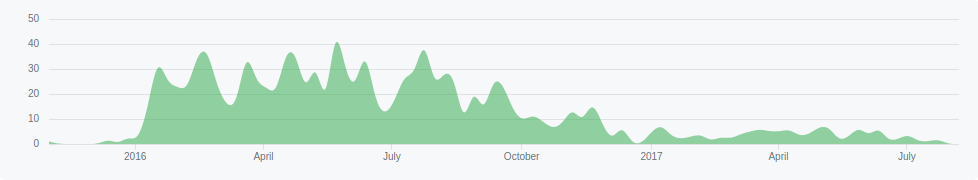
\includegraphics[scale=0.4]{content/pictures/hawkbit_commits.png}
 \caption{Commit-Übersicht des Eclipse hawkBit Sourcecode-Archiv \cite{hawkbit_git}}
 \label{fig:hawkbit_commits}
\end{figure}

In \autoref{tab:rating_hawkbit} sind die wichtigsten Informationen und die Bewertung nochmals in Form eines Steckbriefes zusammengefasst.
\begin{table}[H]
 \centering
 \caption{Steckbrief: Eclipse hawkBit}
 \begin{framed}
 \begin{tabular}{l|l|l|l}
  \multicolumn{4}{l}{}\\
  \multicolumn{4}{l}{\textbf{Eclipse hawkBit}}\\
  \multicolumn{4}{l}{}\\
  \toprule
  %Nr. &  Anforderung & Wertebereich \\
  %\midrule
  \multicolumn{2}{l|}{Webseite des Projektes} & \multicolumn{2}{p{8cm}}{\url{https://eclipse.org/hawkbit/}}\\
  
  \multicolumn{2}{l|}{} & \multicolumn{2}{l}{}\\
  
  \multicolumn{2}{l|}{Beginn der Entwicklung} & \multicolumn{2}{p{8cm}}{September 2015}\\
  
  \multicolumn{2}{l|}{} & \multicolumn{2}{l}{}\\
  
  \multicolumn{2}{l|}{Stand Entwicklung} & \multicolumn{2}{p{8cm}}{Aktuelle Version: 0.2.0M3 vom 03.04.2017} \\
  
  \multicolumn{2}{l|}{} & \multicolumn{2}{l}{} \\
  
  \multicolumn{2}{l|}{Beschreibung} &  \multicolumn{2}{p{8cm}}{
  Bei Eclipse hawkBit handelt es sich um ein recht junges Projekt. Angetrieben wird die Entwicklung hauptsächlich von der 
  Bosch Software Innovations GmbH\footnote{Internetpräsenz Bosch: \url{https://www.bosch-si.com/}}.
  Eclipse hawkBit versteht sich als back-end Framework für das Software Rollout im \ac{IoT}-Umfeld (\ac{IoT}-Inkubator).
  } \\
  
  \multicolumn{2}{l|}{} & \multicolumn{2}{l}{} \\
  
  \multicolumn{2}{l|}{Schwerpunkt} &  \multicolumn{2}{p{8cm}}{
  Der Schwerpunkt liegt auf dem Update- und dem Rollout-Mangement für Gateways und Things im Internet der Dinge.
  Besonderen Wert legen die Entwickler auf eine hohe Skalierbarkeit ihrer Softwarelösung, um ein Software-Rollout auch 
  für eine sehr große Anzahl an Geräten zu ermöglichen.
  } \\
  
  \multicolumn{2}{l|}{} & \multicolumn{2}{l}{} \\
  
  \multicolumn{2}{l|}{Besondere Features} & \multicolumn{2}{p{8cm}}{Kaskadierende Updates von Gruppen, Paket-Modell zur Update-Paketierung, hohe Skalierbarkeit} \\
  
  \multicolumn{4}{l}{} \\
  
  Nr. &  \multicolumn{2}{l|}{Kriterium} & Bewertung \\
  \midrule
  1 & \multicolumn{2}{l|}{Sicherheit}
  & 3 \\
  
  2 & \multicolumn{2}{l|}{Zentrales Management}
  & ja \\
  
  3 & \multicolumn{2}{l|}{Distributionen}
  & ja \\
  
  4 & \multicolumn{2}{l|}{Ausfallsicherheit}
  & ja \\
  
  5 & \multicolumn{2}{l|}{Schnittstellen (\ac{API})}
  & ja \\
  
  6 & \multicolumn{2}{l|}{Zielplattform OSGi}
  & nein \\
  
  7 & \multicolumn{2}{l|}{Existierende Community}
  & ja \\
  
  8 & \multicolumn{2}{l|}{Erkennbare Weiterentwicklung}
  & 2 \\
  
  9 & \multicolumn{2}{l|}{Langlebiges Projekt}
  & 1 \\
  
  10 & \multicolumn{2}{l|}{Flexible Wartbarkeit}
  & 3 \\
  
  11 & \multicolumn{2}{l|}{Anzahl Entwickler}
  & 3 \\
  \bottomrule
 \end{tabular}
 \label{tab:rating_hawkbit}
 \end{framed}
\end{table}

%\footnotetext{Erste Version: \url{https://mvnrepository.com/artifact/org.apache.felix/org.osgi.service.obr/1.0.0}}
Im nächsten Kapitel werden die Einzelbewertungen der Werkzeuge zusammengeführt und es wird eine Entscheidung zugunsten des am besten geeigneten Werkzeuges getroffen.


\section{Entscheidungsmatrix zur Auswahl eines geeigneten Werkzeuges}
\label{sec:matrix}
In diesem Abschnitt wird die Entscheidung über das zum Einsatz kommende Werkzeug getroffen. Dazu werden die Einzelbewertungen aus \autoref{sec:rating} 
in einer Entscheidungsmatrix, siehe \autoref{tab:rating_matrix}, zusammengeführt.
Dabei wurde der Wertebereich ja/nein ebenfalls mit Punkten belegt. Ein ja entspricht vier Punkten und ein nein entspricht einem Punkt.

\begin{table}[h!]
 \centering
 \caption{Entscheidungsmatrix zur Auswahl eines Werkzeuges}
 \resizebox{\columnwidth}{!}{
 \begin{tabular}{l|l||l|l|l|l}
  \multicolumn{6}{l}{}\\
  \multicolumn{6}{l}{\textbf{Entscheidungsmatrix}}\\
  \multicolumn{6}{l}{}\\
  \multicolumn{2}{l||}{Kriterien} & \multicolumn{4}{l}{Werkzeuge}\\
  Nr. & Kriterium & Felix OBR & Apache ACE & Apache Karaf & Eclipse hawkBit \\
  \toprule
  1 & Sicherheit
  & 4 & 3 & 1 & 3 \\
  
  2 & Zentrales Management
  & 1 & 4 & 1 & 4\\
  
  3 & Distributionen
  & 1 & 4 & 4 & 4\\
  
  4 & Ausfallsicherheit
  & 1 & 4 & 1 & 4\\
  
  5 & Schnittstellen (\ac{API})
  & 4 & 4 & 4 & 4\\
  
  6 &  Zielplattform OSGi
  & 4 & 4 & 4 & 1\\
  
  7 & Existierende Community
  & 4 & 4 & 4 & 4\\
  
  8 & Erkennbare Weiterentwicklung
  & 1 & 3 & 4 & 2\\
  
  9 & Langlebiges Projekt
  & 4 & 2 & 3 & 1\\
  
  10 & Flexible Wartbarkeit
  & 4 & 3 & 1 & 3\\
  
  11 & Anzahl Entwickler
  & 2 & 1 & 4 & 3\\
  
  \midrule
  \midrule
  \multicolumn{2}{r||}{$\sum$}
  & 30 & \textbf{36} & 31 & 33 \\
  \bottomrule
 \end{tabular}
 }
 \label{tab:rating_matrix}
\end{table}

%\footnotetext{Erste Version: \url{https://mvnrepository.com/artifact/org.apache.felix/org.osgi.service.obr/1.0.0}}

Die Bewertung zeigt, dass vor allem Apache Felix OBR nur schwer mit den anderen Werkzeugen konkurrieren kann. 
Allerdings hat es auch Stärken im Bereich der Flexibilität und der Verfügbarkeit von Schnittstellen, die den Einsatz dieses Werkzeuges in einem anderen
Anwendungsszenario interessant machen. Apache Karaf überzeugt vor allem durch die hohe Anzahl an Entwicklern und die stetige Weiterentwicklung des Projektes.
Würde Apache Karaf über ein Management-Sub-Projekt verfügen, wäre das Werkzeug ebenfalls im Bereich der Spitzenreiter.
So belegen bei der abschließenden Auswertung die beiden Werkzeuge Apache ACE und Eclipse hawkBit die ersten beiden Plätze.
Die beste Bewertung fällt dabei auf Apache ACE, wobei der Vorsprung nicht sonderlich groß ausfällt.
Für Apache ACE spricht aber momentan noch die Reife der Software, die lange Lebensdauer des Projektes und die Spezialisierung auf \ac{OSGi}.
Sollte Eclipse hawkBit bei seiner Entwicklung wieder eine vergleichbar hohe Aktivität wie zu Beginn des Projektes erreichen,
wird die Bewertung in ein bis zwei Jahren vermutlich zu Gunsten von Eclipse hawkBit ausfallen.\\

Im nächsten Kapitel wird auf Grundlage dieser Bewertung eine prototypische Integration von Apache ACE in das OpenMUC-Framework besprochen.



